\documentclass[10pt,twocolumn,letterpaper]{article}

\usepackage{cvpr}
\usepackage{times}
\usepackage{epsfig}
\usepackage{graphicx}
\usepackage{amsmath}
\usepackage{amssymb}
\usepackage{float}

% Include other packages here, before hyperref.
% If you comment hyperref and then uncomment it, you should delete
% egpaper.aux before re-running latex.  (Or just hit 'q' on the first latex
% run, let it finish, and you should be clear).
\usepackage[breaklinks=true,bookmarks=false]{hyperref}

\cvprfinalcopy % *** Uncomment this line for the final submission

\def\cvprPaperID{****} % *** Enter the CVPR Paper ID here
\def\httilde{\mbox{\tt\raisebox{-.5ex}{\symbol{126}}}}

% Pages are numbered in submission mode, and unnumbered in camera-ready
%\ifcvprfinal\pagestyle{empty}\fi
\setcounter{page}{1}
\begin{document}

%%%%%%%%% TITLE
\title{Automatic Detection of Window Regions in Indoor Point Clouds Using R-CNN}

\author{Craig Hiller, David Zhang, Tianhao Zhang, Zihao Zhang\\
University of California Berkeley\\
{\tt\small \{chiller, dzhang, tianhao.z, geraldzhang\} @ berkeley.edu}
% For a paper whose authors are all at the same institution,
% omit the following lines up until the closing ``}''.
% Additional authors and addresses can be added with ``\and'',
% just like the second author.
% To save space, use either the email address or home page, not both
}

\maketitle
%\thispagestyle{empty}

%%%%%%%%% ABSTRACT
\begin{abstract}
In this paper, we propose an algorithm to automatically identify window regions on exterior-facing building facades in a colored 3D point cloud generated using data captured from an ambulatory backpack sensor system outfitted with multiple LiDAR sensors and cameras. Our work is based on a R-CNN-inspired algorithm, on top on which we added some filtering and preprocessing technique. We use MCG for generating region proposals, pass the proposal to a convolution neural net, and train a random forest with the output vectors. With our implementation, we are able to achieve an F1 score of 89.79\% and mAP of 96.64\%.

\end{abstract}

%%%%%%%%% BODY TEXT
\section{Introduction}

3D modeling of building interior is an important application in the architecture and civil engineering industry. For example, a tool called Energy Plus models and simulates building energy efficiency \cite{rzhang}. In order to model the energy efficiency of a building, it's important to accurately measure the "window to wall ratio" of the exterior facades. In our work, we use data collected by a human-operated backpack-mounted system made of cameras and multi-modal sensors, in order to detect exterior-facing window in the buildings.

Our project branches off of previous work done by Zhang et al. \cite{rzhang} who used the same backpack system as we do. As mentioned in their paper, the task of detecting windows from colored 3D point clouds presents a twofold challenge. Firstly, we are limited by the amount of training data available for structured prediction. Secondly, windows are transparent and are inherently shapeless in 3D space. As a result, conventional image feature descriptors lack discriminative power in identifying windows due to the absence of visual cues such as color and texture. Shape descriptors developed for 3D point clouds are not also applicable \cite{rzhang}. However, our approaches differ substantially in the way we address the aforementioned difficulties and how we leverage the multiple modalities of the data acquisition unit.

In Zhang et al's work, they utilized three features to aid in discriminating between windowed and walled regions. Firstly, they used grayscale intensity values from the visual imaging modality to capture lighting differences between indoor and outdoor regions. Secondly, they measured the proportion of laser-beam returns received by the LiDAR scanner to exploit differences in infrared opaqueness (glass tends to absorb infrared light). Finally, they used a heuristic to construct an "occlusion proxy" feature by noting that occluded regions are more likely to be wall than window \cite{rzhang}.

While the approach proposed by Zhang et al achieves high accuracy and $F_1$ score, their method is limited by some on-site constraints. For example, the grayscale intensity and laser beam reflection feature do not work if the blinds of the window are down, or when the lighting outside the window does not have a strong contrast with the indoor lighting. Our approach attempts to utilize more visual information, which is captured by the left and right camera of the backpack during the data collection. 

We applied the a similar approach to R-CNN\cite{girshick}, with additional processing and fine-tuning, we are able to achieve an accuracy of over 90\%. For each of the images, we generate region candidates, and then for each region proposal, we pass it through a convolution neural net to generate a feature vector. 

This feature vector is then passed through a binary (window or not) classifier that was trained through a similar process. We experimented different algorithms for classification, more details about this will follow in later sections. Since we use learnt feature from the convolution neural net in our detection, our algorithm is more robust to different conditions of indoor and outdoor lighting. Also, we train our classifier with data points sampled from a variety of distributions(daytime and nighttime, blinds up and down etc.) so we are able to detect windows sampled from different environments, adding robustness to our algorithm. The final improvements to our algorithm come from a manual pre-processing of some data in the image set we are classifying. This "human touch" allows us achieve even better results with only a few minutes of human interaction.

%-------------------------------------------------
\section{Algorithm Description}

% This is a graph that illustrates the entire algorithm
\begin{figure*}[t!]
\centering
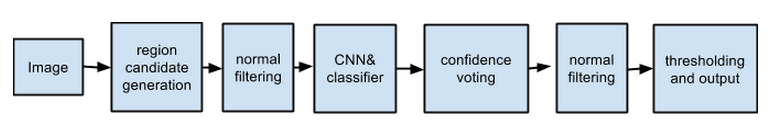
\includegraphics[width=0.9\textwidth]{plots/pipeline.png}
\caption{pipeline}
\end{figure*}

\subsection{Ground Truthing}
Since there are no substantial datasets of windows with their precise regions labeled, we need to generate our own labels for existing images. Because we needed both images to test and train on, we manually labeled approximately 1200 images from our Mulford Hall dataset, 400 images from the Cory Hall dataset, as well as pulled images from Google Images and captured around 40 pictures of windows around the UC Berkeley campus. For each of the images, our tool for hand-labeling generates a binary mask where the mask has value one where there's window and zero otherwise. These images and masks are used as the basis of the experiments used in the rest of the paper. An example is shown in Figure 3.

\subsection{Region Candidate Generation}
% Started with selective-search, changed to MCG
We initially started with selective search to generate candidate regions, but we found that using multiscale combinatorial grouping (MCG) \cite{mcg} gave us better proposals, at the expense of more slightly more computation per image. The output of this stage gives us a set of region proposals (roughly 2000 per image) along with their respective bounding boxes. Each region proposal is extracted "without context", i.e. we exclude the background image content outside of the proposal. These regions are then used for feature extraction.


\subsection{Feature Extraction}

We use R-CNN to extract a 4096-dimensional feature vector from each region proposal generated by MCG. The CNN used is a Caffe implementation of AlexNet \cite{alexnet} except the order of normalization and pooling layers is swapped, and training was performed without dataset augmentation. Each region proposal is forward propagated through five convolutional layers and two fully connected layers to generate a feature vector. That is, we take the output of the final hidden layer (\textit{fc7}) of the network as our feature vector.

The input to the CNN is a $256\times256$ RGB image, so we simply scale the input via interpolation to fit these dimensions. Alternative methods include "tightest box with context" and anisotropic scaling methods, as discussed in Appedix A of \cite{girshick}.

\subsection{Classification}
% Random forest vs. SVM

We experimented with using a linear SVM and a random forest to perform binary classification. We used our ground truth dataset to cross-validate each method using grid search to determine the optimal hyper-parameters for each model.


A random forest consisting of 100 trees gave us the best results with 91.7\% validation accuracy. With an SVM, we were able to achieve comparable performance (90.1\% validation accuracy) after scaling our features to have zero mean and unit variance. In addition to offering better validation accuracy, using random forests also enabled us to reduce the amount of time spent on training through parallelization. For 100 trees, training took less than 13 seconds when parallelized across 18 cores of an Intel Xeon CPU 3.1GHz CPU. Although the SVM would probably scale better at test time for very large datasets, we choose to use a random forest for its slightly better performance and ease of integration with our system.



\subsection{Evaluation}
% Normal map filtering
At test time for each of the test images, we follow the pipeline that we described earlier in this section. We generate region candidate proposals, apply a filter to the proposal using surface normal information generated from the laser data collected by the backpack system. More detail about the normal map will be specified below. After the filtering, we pass the region candidates through the convolution neural net and get the feature vector, run all the vectors through our classifier. Once we have all the positive candidate from the classifier, we perform a confidence voting on a binary mask, more details below. In the end, we threshold the mask to get the window area. Figure 1 is a visualization of our pipeline.



 
\subsubsection{Normal Map filtering}
With the normal map filtering, we exploit the fact that windows are located on the walls inside a building, we eliminate the region candidates that has a surface normal facing down or facing up. The normal map we generate contains the normal unit vector of the surface at each pixel, so we can use the information to help us determine whether a region candidate is valid or not. After the filtering, we are able to reduce the run-time of the CNN and classification stage. We are able able to reject candidates that are on the ceilings and floor, but could be confused with windows. In Figure 2, we show the region candidates generated without filtering, the corresponding normal map, and the region candidates after filtering.

\begin{figure*}
\begin{center}
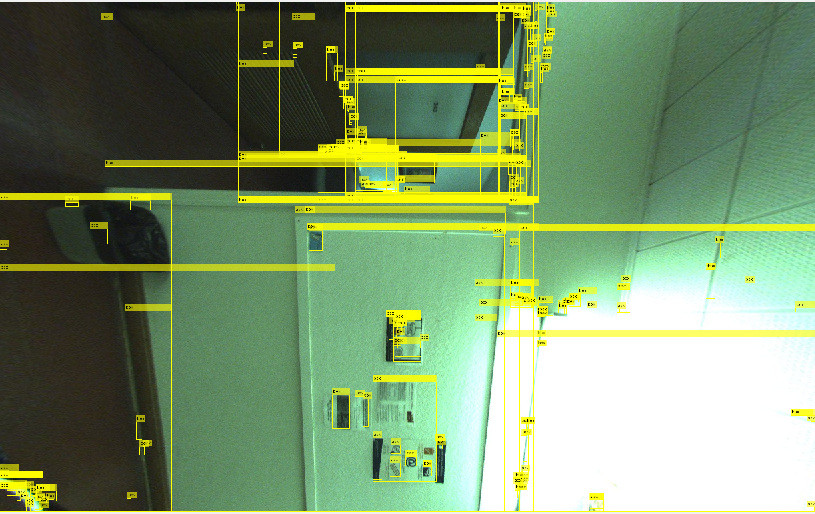
\includegraphics[width=0.4\textwidth,angle=90]{plots/303wo.png}
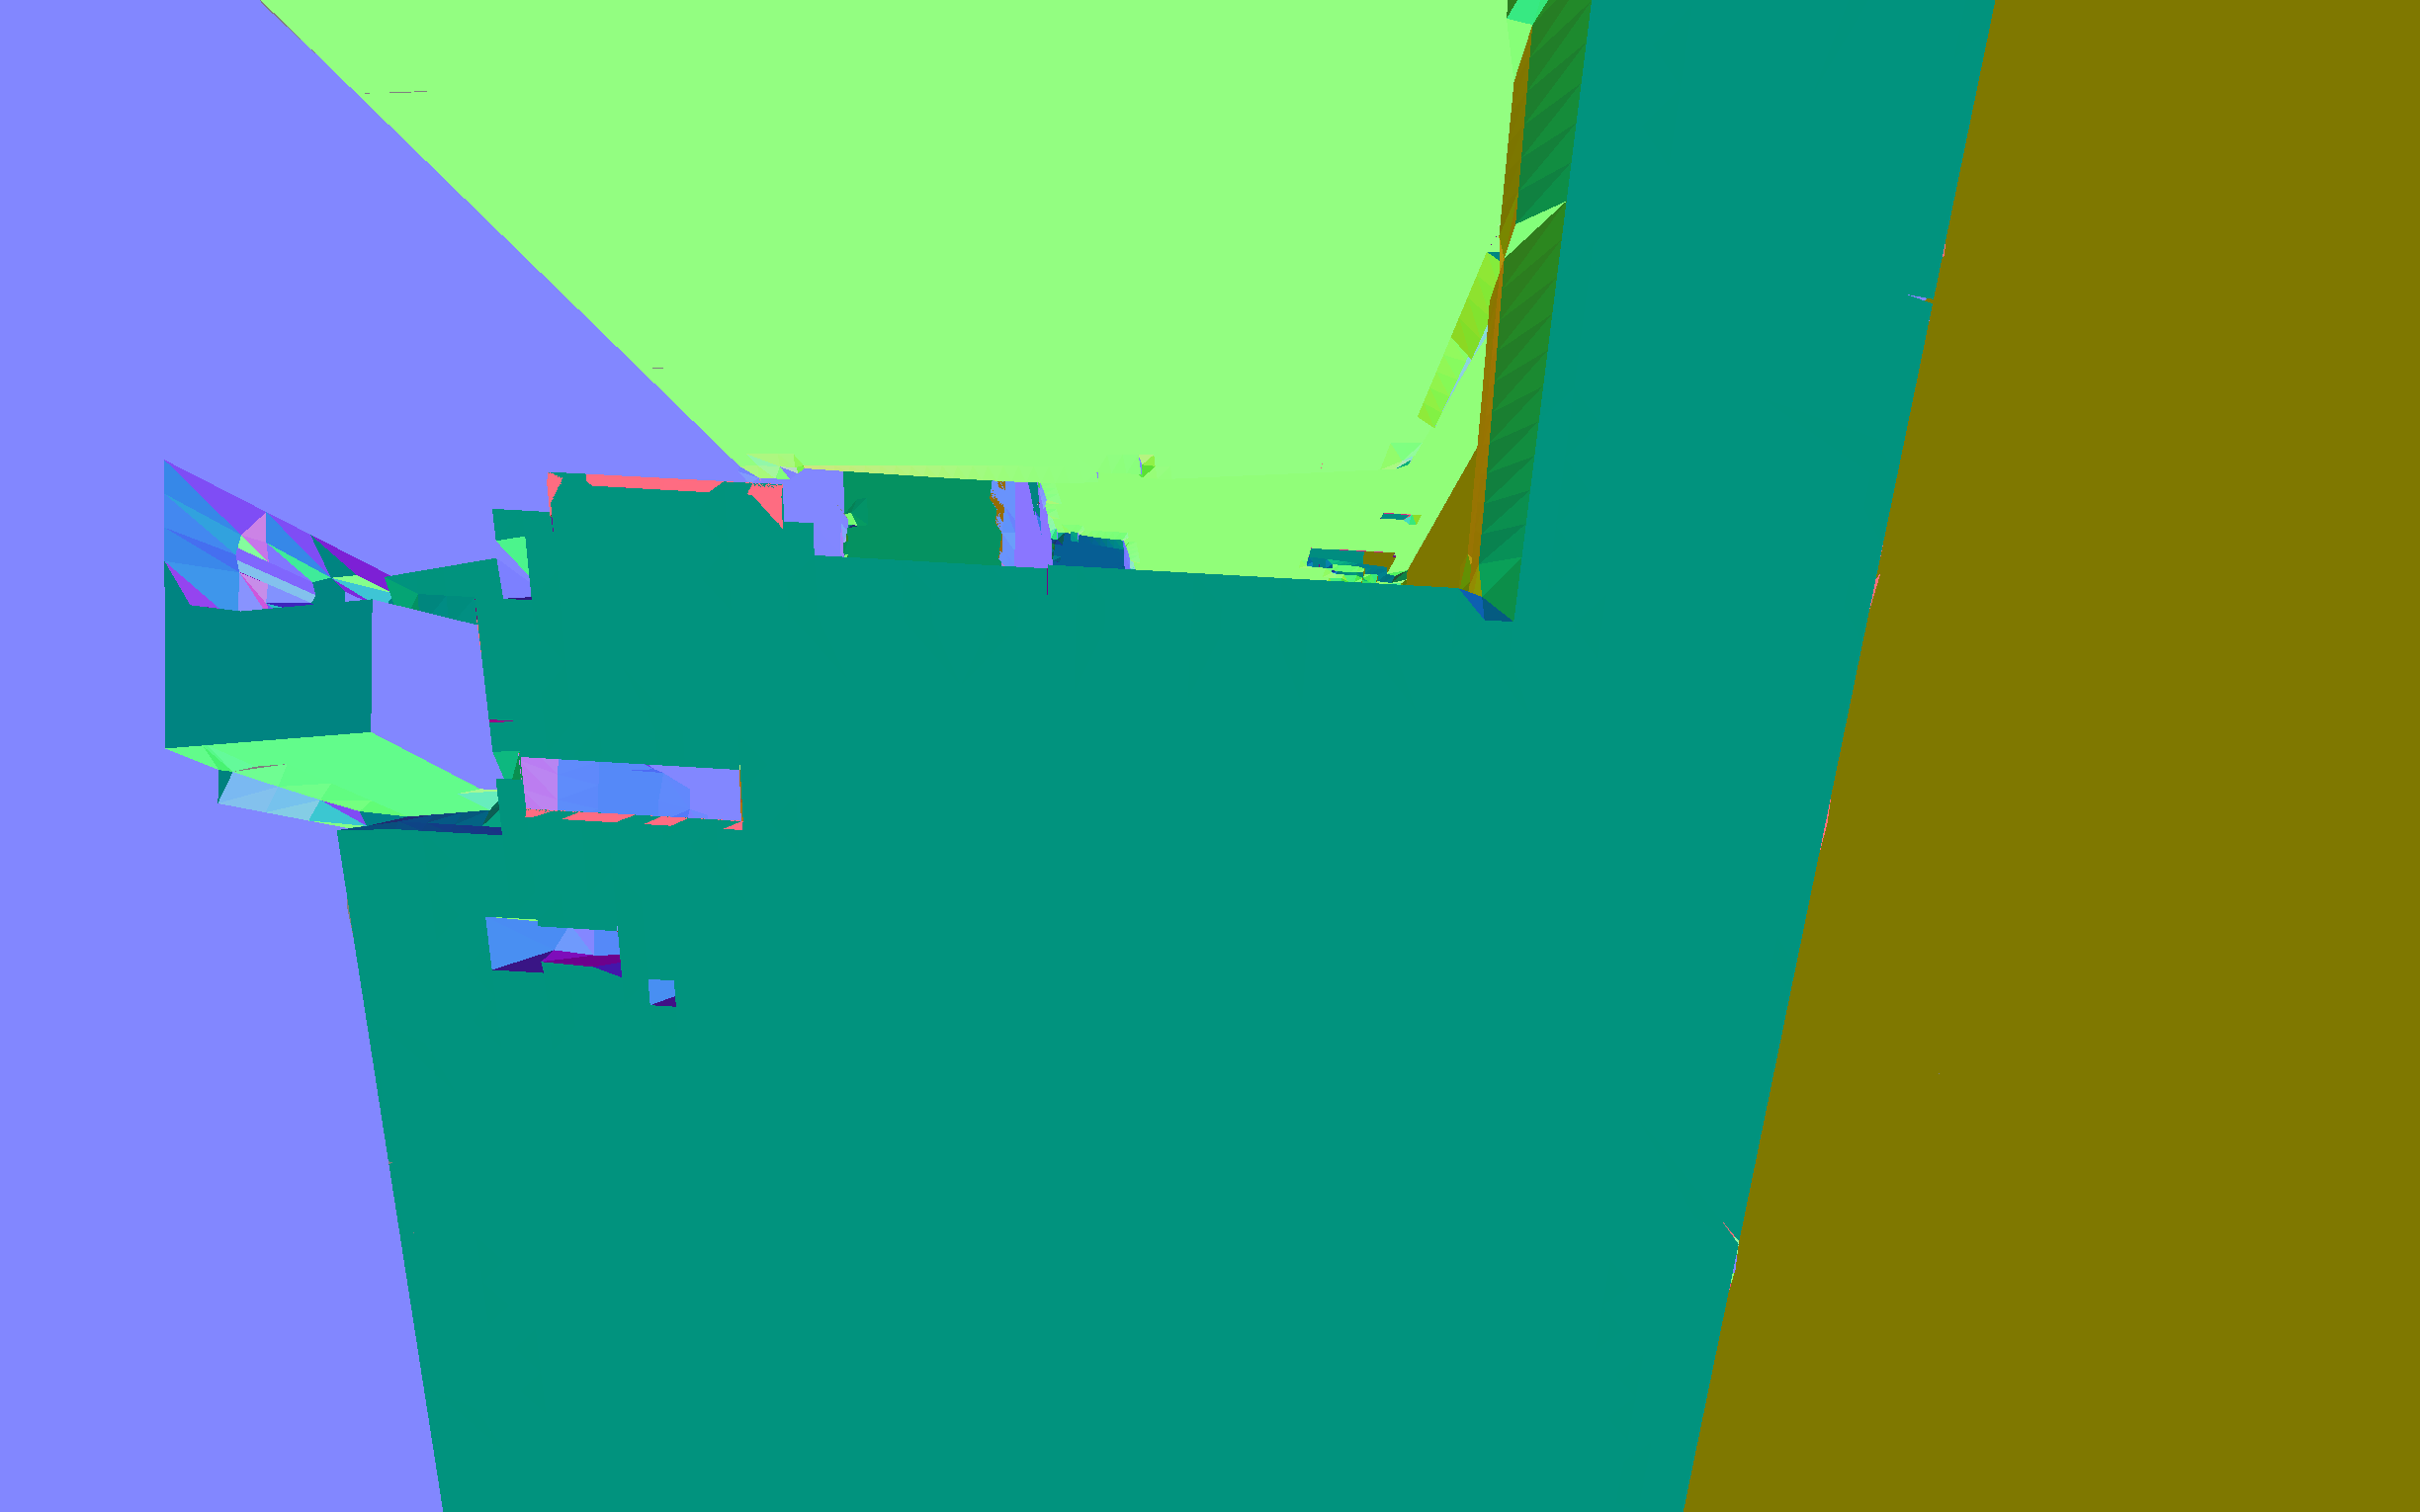
\includegraphics[width=0.4\textwidth,angle=90]{plots/normal.png}
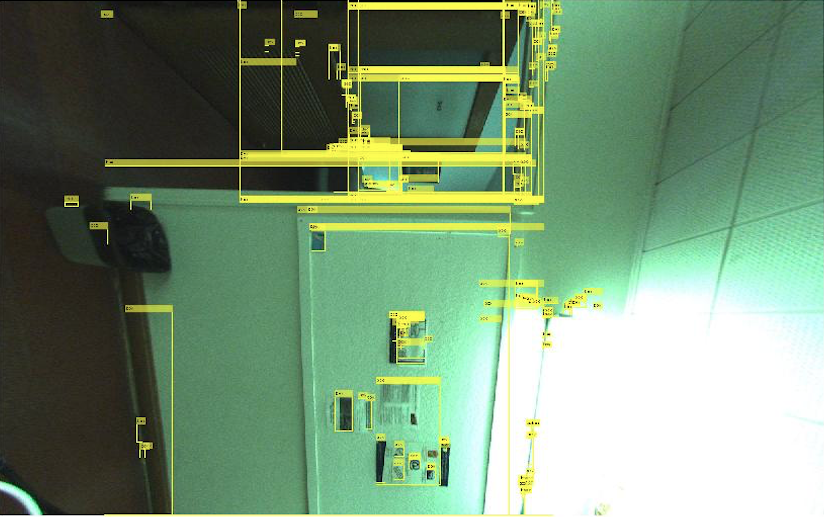
\includegraphics[width=0.4\textwidth,angle=90]{plots/303w.png}
\end{center}
\caption{region candidates generated without filtering, the correspondent normal map, and the region candidates after filtering}
\end{figure*}

\subsubsection{Confidence Voting}
Once we have the positive candidates returned from the classifier, we want to generate a binary mask for denoting the regions that our algorithm would classify as windows. 

We experienced with an naive algorithm such that for each pixel, if the pixel is contained in any positive region candidate mask, we classify that pixel as window area. However, although we have an over 90 percent cross-validation accuracy for our classifier, false positives have significant impact on the outcome of the naive algorithm. A example is shown in Figure 3.

To overcome this problem, we implemented a voting based algorithm. We begin with an all-zero gray-scale mask, and then for each region candidate mask, we add some confidence score to the gray-scale mask. Since window is a continuous-shaped object, we penalize the region proposals with large bounding boxes but small masks.

For each region candidate
\begin{equation}
\mathrm{confidence\ score} = e^{r}-1
\end{equation}
where $r$ is the proportion of the bounding box area to mask area.

Since the result gray-scale image should be invariant to the number of positive bounding boxes, we normalize the gray-scale mask to [0, 1].

After we apply the confidence voting, the resulting gray-scale map has much better accuracy. A comparison of the naive result and the confidence voting result is shown in figure 3 below.

\begin{figure}[h]
\centering
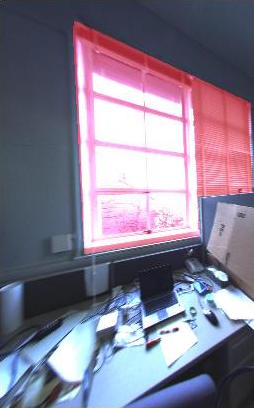
\includegraphics[width=0.2\textwidth]{plots/eg1_original.jpg}
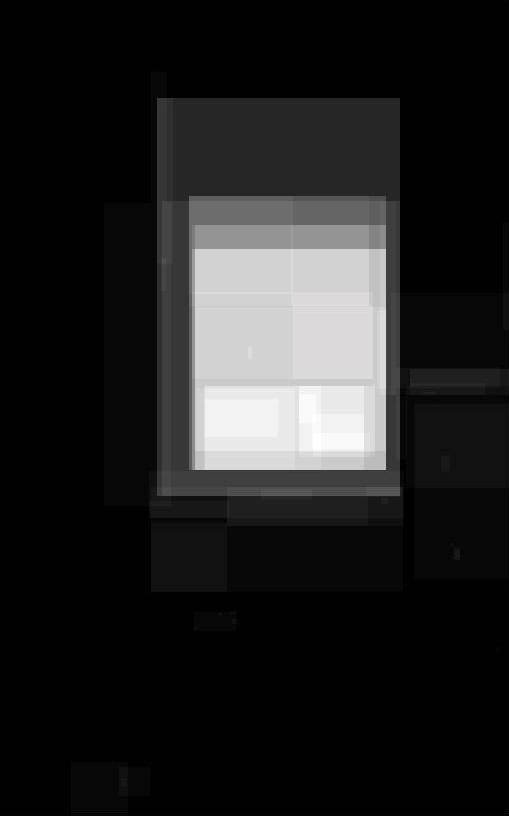
\includegraphics[width=0.2\textwidth]{plots/generalDataDF.jpg}
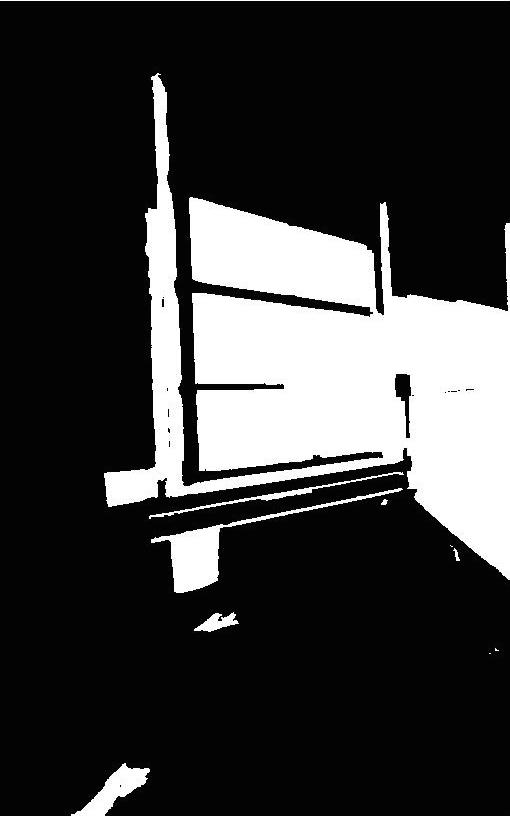
\includegraphics[width=0.2\textwidth]{plots/eg1_naive.jpg}
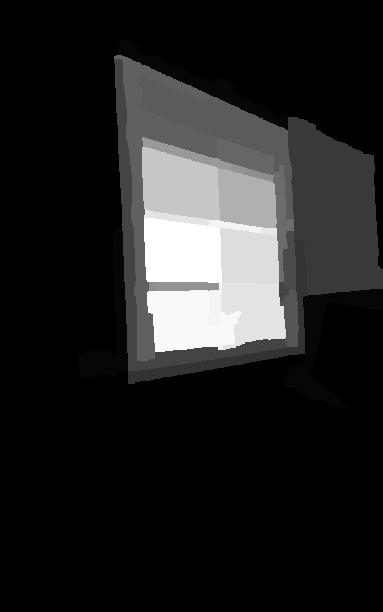
\includegraphics[width=0.2\textwidth]{plots/eg1_conf.jpg}
\caption{test image with ground truth shaded (upper left), non-human augmented classification with confidence voting (upper right) human-augmented with no confidence voting result (lower left) and the confidence voting result with human augmented dataset (bottom right)}
\end{figure}


\begin{figure}[b]
\centering
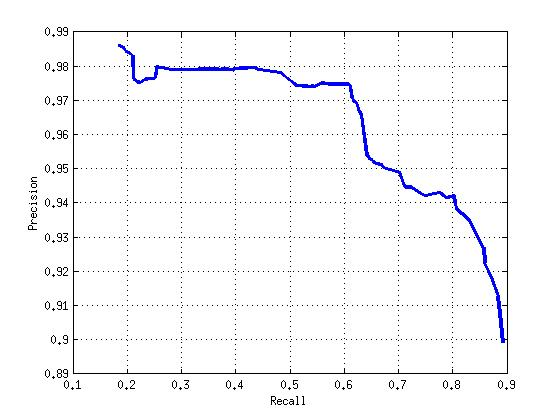
\includegraphics[width=0.45\textwidth]{plots/pr.jpg}
\caption{precision recall curve}
\end{figure}


\subsection{Human Augmented Dataset}
Using just images collected from Google Images and taken around campus, the window regions we detect tend to miss the blinds. This is in part due to a lack of curtained or blinded image data in that training dataset, and when we enter a new environment, we may encounter a type of window covering we may have not seen before. Having a human label a small fraction of randomly chosen images from the images we are trying to classify gives our algorithm a stronger sense of the window and blind types in the overall dataset. This relies on the assumption that in a given building a general style is preserved and randomly picking images should cover most of the variation. In our experiment we used 40 images, which took less than ten minutes to classify. The improvement of adding in this new data is shown in Figure 3.  

\section{Experiment Results}
We ran our software on the dataset that we collected using the backpack on the third floor of Cory Hall, The test set contains 400 images with hand labeled ground truth. We achieved an $F_1$ score of 89.79\% (P:91.27, R:88.35) and mAP of 96.64\% compared to the 85.5 $F_1$ score and 94.2\% mAP achieved by the method proposed by Zhang et al \cite{rzhang}. 

The method used by Zhang et al. had difficulty detecting windows occluded by blinds, curtains, and other objects. We found that our method was able to successfully capture these regions, which we attribute to our ability to exploit the visual imaging modality of our sensor system.

\section{Conclusion and Future Work}

We believe that our R-CNN approach gives us results competitive with those of Zhang et al. Our method has also has a lot of potential for future refinement. In particular, we did not perform any fine-tuning of our CNN with domain specific data as in \cite{girshick}. We also believe that a larger ground truth dataset would allow our method to generalize better. Another way to improve the result of the window detector would be augmenting our algorithm with the some of the work that Zhang et al. done, and make our result onto a 3D point cloud model to calculate the "window to wall ratio".


For inspirations outside of this task, we could also generalize the concept of confidence voting and apply it to general object recognition.


{\small
\bibliographystyle{ieee}
\bibliography{egbib}
}

\end{document}